% 第1章第2节：线性递推的求解（常系数递推与矩阵幂；时变递推与状态转移）。

\section{线性递推的求解}
\label{sec:dds-linear-recurrences}

一般的非线性递推只能逐步计算。线性和仿射更新则不同：叠加原理让我们把轨迹拆成“初态单独传播”与“每次输入单独传播”两部分，各自写成显式公式。本节先处理系数不随时间变化的情形，这时初态的作用由矩阵幂决定，矩阵的特征值告诉我们各个方向是增长、衰减还是旋转；再处理时变系数，这时必须保留矩阵乘积的先后次序。

\subsection{常系数递推与矩阵幂}
\label{sec:dds-constant-coefficient}

\paragraph{从等比数列到矩阵幂}
最简单的线性递推是标量的$x_{n+1}=ax_n$，它的解是等比数列$x_n=a^nx_0$。$|a|<1$时状态几何衰减，$|a|>1$时几何增长，$a<0$时每步变号，形成来回摆动。温度偏差$x_n-2=0.8^n(x_0-2)$正是$a=0.8$的情形。

向量情形$\bm x_{n+1}=\bm A\bm x_n$的解同样直接：$\bm x_n=\bm A^n\bm x_0$。困难在于读懂$\bm A^n$。矩阵幂的元素一般不是原矩阵元素的幂，例如$\bigl[\begin{smallmatrix}1&1\\0&1\end{smallmatrix}\bigr]^n=\bigl[\begin{smallmatrix}1&n\\0&1\end{smallmatrix}\bigr]$，右上角线性增长，而原矩阵的元素都只有$0$和$1$。要理解长期行为，需要找到让$\bm A$作用变简单的方向。

\paragraph{特征方向：增长、衰减与旋转}
若$\bm A\bm v=\lambda\bm v$，从$\bm v$出发的轨道就是$\lambda^n\bm v$：在特征方向上，矩阵递推退化为标量的等比数列。当$\bm A\in\mathbb R^{d\times d}$有$d$个线性无关的特征向量$\bm v_1,\ldots,\bm v_d$时，把初值分解为$\bm x_0=\sum_ic_i\bm v_i$，得到
\begin{equation}
  \bm x_n=\sum_{i=1}^dc_i\lambda_i^n\bm v_i .
  \label{eq:dds-modal-solution}
\end{equation}
每个分量各自按自己的倍数伸缩，互不干扰。长期看，模最大的特征值主导，只要初值在它的方向上有分量。

想象把所有长度为$1$的初值画成单位圆，再看$\bm A^n$把这个圆变成什么。图~\ref{fig:dds-matrix-power-shapes}(a)中，$\bm A$在水平方向有特征值$1.25$，在对角方向有特征值$0.6$。单位圆被反复作用后，沿水平方向越拉越长，沿对角方向越压越扁，变成一个越来越细长、并逐渐倒向水平特征方向的椭圆。长期看，几乎每个初值都会被拉向增长方向，只有恰好落在对角特征方向上的初值才会衰减到零。

\begin{figure*}[htbp]
  \centering
  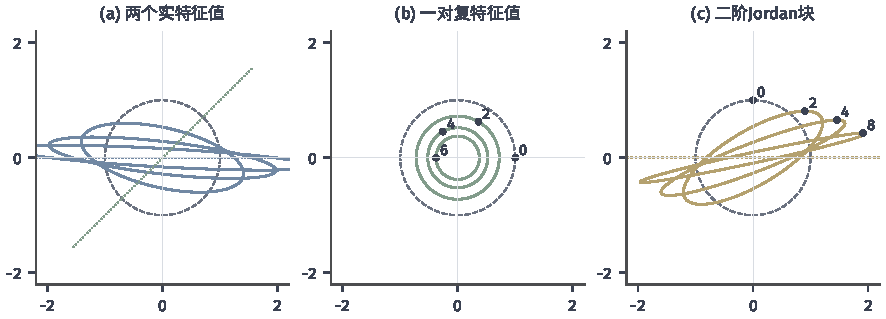
\includegraphics[width=150mm]{figures/03-optimization-evolution-and-signals/02-processes-and-trajectory-evolution/matplotlib/dds-matrix-power-shapes/figure.pdf}
  \caption{矩阵幂对单位圆的作用。虚线为单位圆，实线为它在$\bm A^n$下的像。(a)$\bm A$在水平方向$(1,0)^{\top}$有特征值$1.25$、在对角方向$(1,1)^{\top}$有特征值$0.6$（点线），画$n=1,2,3$：圆被拉长并压扁，倒向增长方向。(b)$\bm A=0.85\,\bm R(\pi/6)$，$\bm R(\varphi)$为逆时针旋转$\varphi$，特征值$0.85\mathrm e^{\pm\mathrm i\pi/6}$，画$n=2,4,6$：圆保持为圆，边旋转边收缩，黑点是$(1,0)^{\top}$的像。(c)$\bm A=\bigl[\begin{smallmatrix}0.9&0.5\\0&0.9\end{smallmatrix}\bigr]$只有一个特征方向（水平点线），画$n=2,4,8$：圆被剪切成斜椭圆，黑点$(0,1)^{\top}$的像先向右远离再缓慢回收。}
  \label{fig:dds-matrix-power-shapes}
\end{figure*}

实矩阵的特征值可以是复数，对应的几何是旋转。设$\lambda=r\mathrm e^{\mathrm i\varphi}$（$r>0$，$0<\varphi<\pi$）是$\bm A$的特征值，复特征向量为$\bm v=\bm p+\mathrm i\bm q$，$\bm p,\bm q\in\mathbb R^d$。比较$\bm A\bm v=\lambda\bm v$两边的实部和虚部，得到
\[
  \bm A\bm p=r(\cos\varphi\,\bm p-\sin\varphi\,\bm q),\qquad
  \bm A\bm q=r(\sin\varphi\,\bm p+\cos\varphi\,\bm q).
\]
因此$\bm p,\bm q$张成的平面在$\bm A$下不变，而在基$(\bm p,\bm q)$下，$\bm A$的作用是把坐标旋转角度$\varphi$（方向由基的取向决定）再乘以$r$。反复作用得到旋转$n\varphi$、缩放$r^n$：轨道沿螺线走向原点（$r<1$）或远离原点（$r>1$）。图~\ref{fig:dds-matrix-power-shapes}(b)是最干净的情形，$\bm A$本身就是$0.85$乘以旋转$\pi/6$。

第~\ref{sec:dds-recurrence-state}小节的动量迭代~\eqref{eq:dds-heavy-ball-state}正是这种情形：它的矩阵没有实特征向量，只有一个旋转缩放的不变平面。

\begin{example}[动量迭代的振荡收敛]
\label{ex:dds-heavy-ball-oscillation}
矩阵$\bigl[\begin{smallmatrix}0.9&-0.4\\1&0\end{smallmatrix}\bigr]$的特征多项式是$\lambda^2-0.9\lambda+0.4$，判别式$0.81-1.6<0$，两根$\lambda=0.45\pm0.4444\mathrm i$。它们的模$r=\sqrt{0.4}\approx0.632$等于两根之积（行列式）的平方根，辐角$\varphi=\arccos(0.45/\sqrt{0.4})\approx44.6^{\circ}$。于是参数$\theta_n$可写成$r^n(C_1\cos n\varphi+C_2\sin n\varphi)$：每步大约转过$45^{\circ}$，约$8$步完成一次振荡，同时振幅每步乘以$0.632$。动量让迭代越过最小点再折回，这在矩阵层面就是一对复特征值。
\end{example}

\paragraph{不可对角化时的多项式因子}
特征向量不够$d$个时，分解~\eqref{eq:dds-modal-solution}不可用，矩阵幂中会出现多项式因子。二维情形已经包含全部机制。考察
\[
  \bm J=\begin{bmatrix}\lambda&1\\0&\lambda\end{bmatrix},\qquad
  \bm J^n=\begin{bmatrix}\lambda^n&n\lambda^{n-1}\\0&\lambda^n\end{bmatrix}.
\]
右式用归纳法验证：$\bm J^n\bm J$的右上角是$\lambda^n+n\lambda^{n-1}\cdot\lambda=(n+1)\lambda^n$。$\bm J$只有一个特征值$\lambda$，而$\bm J-\lambda\bm I$的秩为$1$，所以只有一个特征方向$(1,0)^{\top}$。这样的矩阵称为二阶\term{Jordan块}（Jordan block）。第二个坐标的初值会通过右上角的$1$持续“推”第一个坐标，累计出因子$n$。

多项式因子不会改变最终是增长还是衰减，只改变途中的形状。$|\lambda|<1$时，$n|\lambda|^{n-1}\to0$，因为几何衰减终将压过线性增长；但起初$n$的增长可能占上风。图~\ref{fig:dds-matrix-power-shapes}(c)中$\lambda=0.9$，点$(0,1)^{\top}$的像依次是$(0.5n\cdot0.9^{n-1},\,0.9^n)$：$n=2,4,8$时横坐标约为$0.90$、$1.46$、$1.91$，先远离原点，很久以后才回收。$|\lambda|=1$时多项式因子决定一切：$\lambda=1$给出$\bm J^n=\bigl[\begin{smallmatrix}1&n\\0&1\end{smallmatrix}\bigr]$，特征值的模不超过$1$，矩阵幂却无界。

调整动量迭代的参数，可以让一对复特征值合并成二重实根，恰好落到这种不可对角化的情形。

\begin{example}[临界阻尼的动量迭代]
\label{ex:dds-critical-damping}
把参数改为$\eta=\beta=0.25$，递推成为$\theta_{n+1}=\theta_n-0.25\,\theta_{n-1}$，特征多项式$\lambda^2-\lambda+0.25=(\lambda-0.5)^2$有二重根$0.5$，而相应矩阵$\bigl[\begin{smallmatrix}1&-0.25\\1&0\end{smallmatrix}\bigr]$减去$0.5\bm I$后秩为$1$，只有一个特征方向。直接代入可验证$\theta_n=(c_1+c_2n)\,0.5^n$满足递推：对$\theta_n=n\,0.5^n$，
\[
  \begin{aligned}
  &(n+1)0.5^{n+1}-n\,0.5^n+0.25(n-1)0.5^{n-1}\\
  &\quad=0.5^n\bigl[0.5(n+1)-n+0.5(n-1)\bigr]=0 .
  \end{aligned}
\]
这是“临界阻尼”：复根刚好合并成实二重根，振荡消失，留下一个多项式因子。
\end{example}

一般矩阵可以相似变换成若干Jordan块组成的分块对角形，所以$\bm A^n$的元素总是形如$n^k\lambda^n$的项的线性组合，其中$k$小于相应块的阶数。本章不需要这一完整理论，只用下面的估计。卷一已经证明：对任意$r>\rho(\bm A)$，其中$\rho(\bm A)=\max\{|\lambda|:\lambda\text{为}\bm A\text{的特征值}\}$是\term{谱半径}（spectral radius），存在常数$C_r\geq1$，使
\begin{equation}
  \lVert\bm A^n\rVert\leq C_r\,r^n,\qquad n\geq0,
  \label{eq:dds-geometric-bound}
\end{equation}
等价地，存在$\mathbb R^d$上的一个向量范数，使$\bm A$在它诱导的矩阵范数下不超过$r$。卷一还证明了$\bm A^n\to\bm 0$当且仅当$\rho(\bm A)<1$，以及$\rho(\bm A)=\lim_{n\to\infty}\lVert\bm A^n\rVert^{1/n}$（Gelfand公式）。证明用实Schur形把矩阵化成准上三角形，再用对角缩放把非对角块压小；常数$C_r$正是吸收多项式因子与非正交特征方向的代价，$r$越接近$\rho(\bm A)$，$C_r$可能越大。这些结论与证明可参考\BookChapterRef{chap:linear-analysis}{卷一“谱和奇异值”章}。

\paragraph{输入的累计：注入时刻与剩余传播}
现在加上输入。对常系数系统$\bm x_{n+1}=\bm A\bm x_n+\bm B\bm u_n$，前两步是
\[
  \bm x_1=\bm A\bm x_0+\bm B\bm u_0,\qquad
  \bm x_2=\bm A^2\bm x_0+\bm A\bm B\bm u_0+\bm B\bm u_1 .
\]
规律已经显现：较早的输入被多乘了几次$\bm A$。

\begin{theorem}[常系数仿射递推的显式解]
\label{thm:dds-variation-constants}
设$\bm A\in\mathbb R^{d\times d}$、$\bm B\in\mathbb R^{d\times m}$，$\bm x_0\in\mathbb R^d$，$(\bm u_n)\subseteq\mathbb R^m$。递推$\bm x_{n+1}=\bm A\bm x_n+\bm B\bm u_n$的解为
\begin{equation}
  \bm x_n=\bm A^n\bm x_0+\sum_{j=0}^{n-1}\bm A^{\,n-1-j}\bm B\bm u_j,\qquad n\geq0,
  \label{eq:dds-variation-constants}
\end{equation}
其中$n=0$时求和为空，取零向量。
\end{theorem}

\begin{proof}
$n=0$时右边为$\bm x_0$。设式~\eqref{eq:dds-variation-constants}对某个$n$成立，则
\[
  \begin{aligned}
  \bm x_{n+1}=\bm A\bm x_n+\bm B\bm u_n
  &=\bm A^{n+1}\bm x_0+\sum_{j=0}^{n-1}\bm A^{\,n-j}\bm B\bm u_j+\bm A^0\bm B\bm u_n\\
  &=\bm A^{n+1}\bm x_0+\sum_{j=0}^{n}\bm A^{\,(n+1)-1-j}\bm B\bm u_j .
  \end{aligned}
\]
这正是$n+1$时的公式。
\end{proof}

公式的每一项都有一个“注入—传播”的读法。输入$\bm u_j$在第$j$步注入状态，变成$\bm B\bm u_j$；此后到时刻$n$还要经历$n-1-j$次更新，每次乘以$\bm A$。所以$\bm A^{\,n-1-j}\bm B\bm u_j$是“$j$时刻注入、传播$n-1-j$步”后的残余，状态$\bm x_n$是全部残余与初态残余$\bm A^n\bm x_0$的叠加。图~\ref{fig:dds-input-injection}把标量情形$a=0.8$画成堆叠的面积：每次加热都激起一条按$0.8^k$衰减的“余波”，各条余波叠起来恰好是递推算出的温差。

\begin{figure}[htbp]
  \centering
  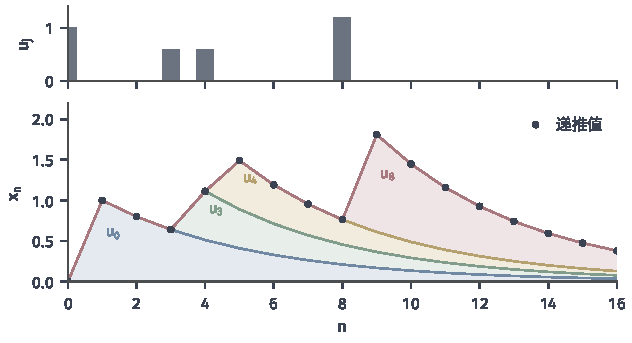
\includegraphics[width=107mm]{figures/03-optimization-evolution-and-signals/02-processes-and-trajectory-evolution/matplotlib/dds-input-injection/figure.pdf}
  \caption{输入的注入与剩余传播。上图为输入序列：$u_0=1$，$u_3=u_4=0.6$，$u_8=1.2$，其余为$0$。下图对$x_{n+1}=0.8x_n+u_n$、$x_0=0$，把每个非零输入的贡献$0.8^{\,n-1-j}u_j$按颜色堆叠；第$j$个输入从$n=j+1$开始出现，此后每步乘以$0.8$。黑点是直接递推得到的$x_n$，与各层之和逐点相同。}
  \label{fig:dds-input-injection}
\end{figure}

公式中“较早的输入被多乘几次$\bm A$”的读法，可以用一个三步的小例子直接核对。

\begin{example}[注入—传播的数值核对]
\label{ex:dds-injection-check}
取$a=1/2$、$b=1$、$x_0=0$，输入$u_0=1$、$u_1=2$、$u_2=1$。逐步递推得$x_1=1$、$x_2=5/2$、$x_3=9/4$。按公式，$x_3=a^2u_0+a\,u_1+u_2=\frac14+1+1=\frac94$：最早的输入传播了两步，只剩四分之一。
\end{example}

零初态时，式~\eqref{eq:dds-variation-constants}是输入序列与固定序列$\bm H_k=\bm A^k\bm B$的离散\term{卷积}（convolution）：$\bm x_n=\sum_{j=0}^{n-1}\bm H_{n-1-j}\bm u_j$。$\bm H_k$描述“单位输入在$k$步以前注入、如今还剩多少”，称为从输入到状态的\term{脉冲响应}（impulse response）。若再读出$\bm y_n=\bm C\bm x_n$，输入到输出的脉冲响应就是$\bm C\bm A^k\bm B$。从卷积和频率的角度研究这种输入—输出关系，是第~\ref{chap:signal-analysis}章的任务；这里只需注意，非零初态的自由响应$\bm A^n\bm x_0$不在卷积之内，必须另外加上。

\paragraph{恒定输入与平衡偏移}
输入恒定为$\bm u$时，若$1$不是$\bm A$的特征值，则$\bm I-\bm A$可逆，方程$\bm x_*=\bm A\bm x_*+\bm B\bm u$有唯一解
\begin{equation}
  \bm x_*=(\bm I-\bm A)^{-1}\bm B\bm u .
  \label{eq:dds-forced-equilibrium}
\end{equation}
用它平移坐标，$\bm x_{n+1}-\bm x_*=\bm A\bm x_n+\bm B\bm u-(\bm A\bm x_*+\bm B\bm u)=\bm A(\bm x_n-\bm x_*)$，所以
\[
  \bm x_n=\bm x_*+\bm A^n(\bm x_0-\bm x_*).
\]
温度例中$x_*=0.4/(1-0.8)=2$，与第~\ref{sec:dds-recurrence-state}小节的计算一致。当$\rho(\bm A)<1$时$\bm A^n\to\bm0$，初态的影响消失，轨迹趋于$\bm x_*$；但$\bm x_*$一般不是零。“初态衰减”与“状态趋零”是两回事：前者只说明系统忘记了从哪里出发，持续施加的输入仍然把状态维持在偏离原点的位置。若$1$是$\bm A$的特征值，平衡可能不存在：标量$a=1$时$x_n=x_0+nu$，任何非零恒定输入都使状态线性增长。

指数移动平均是这一结构的常用实例。递推~\eqref{eq:dds-ema}中令$a=1-\alpha$，由式~\eqref{eq:dds-variation-constants}（时刻从$1$开始计）得
\begin{equation}
  m_n=a^nm_0+\alpha\sum_{j=1}^na^{\,n-j}u_j .
  \label{eq:dds-ema-expansion}
\end{equation}
初值与各次输入的权重之和为$a^n+\alpha(1-a^n)/(1-a)=1$，所以$m_n$是一个加权平均。$k$步以前的输入权重是$\alpha a^k$，降到当前输入权重的$\mathrm e^{-1}$所需的步数为$-1/\ln(1-\alpha)$，$\alpha$较小时约为$1/\alpha$：$\alpha=0.1$时约$9.5$步，$\alpha=0.2$时约$4.5$步。若$m_0=0$只表示“尚无数据”，有限步内观测项的权重之和只有$1-a^n$，把$m_n$除以$1-a^n$可以重新归一化；若$m_0$本身是有效的初始估计，这样做会改变原定的更新。

恒定输入下的平衡还能说明EMA跟踪变化量时的滞后。设输入是匀速上升的$u_j=\mu_0+jd$，记偏差$b_n=m_n-u_n$。由$m_n=am_{n-1}+\alpha u_n$与$u_n=u_{n-1}+d$，
\[
  b_n=a\,m_{n-1}+\alpha u_n-u_n=a\,(m_{n-1}-u_{n-1})-a\,d=a\,b_{n-1}-a\,d .
\]
这是一个系数为$a$、恒定输入为$-ad$的标量递推，平衡为$b_*=-ad/(1-a)=-ad/\alpha$。$\alpha=0.2$时，平均值长期落后真实值$4d$。$\alpha$越小，记忆越长、平滑越强，滞后也越大；平滑与跟踪之间的取舍，在这里成了同一个递推的平衡位置。

\subsection{时变递推与状态转移}
\label{sec:dds-time-varying}

\paragraph{按时间排序的状态转移矩阵}
系数随时间改变时，$\bm x_{n+1}=\bm A_n\bm x_n+\bm B_n\bm u_n$的齐次部分不再是同一个矩阵的幂，而是一串不同矩阵的乘积。为记录“从时刻$m$到时刻$n$”的传播，定义
\begin{equation}
  \bm\Phi(n,m)=\bm A_{n-1}\bm A_{n-2}\cdots\bm A_m\quad(n>m),\qquad
  \bm\Phi(m,m)=\bm I ,
  \label{eq:dds-transition-matrix}
\end{equation}
称为\term{状态转移矩阵}（state transition matrix）。约定$\bm\Phi(m,m)=\bm I$是空乘积的自然取值：不经历任何更新，状态不变。较晚的矩阵写在左边，与复合映射的顺序一致。

由定义直接得到三条性质：$\bm\Phi(n+1,m)=\bm A_n\bm\Phi(n,m)$；对$m\leq k\leq n$有$\bm\Phi(n,m)=\bm\Phi(n,k)\bm\Phi(k,m)$，即先从$m$传播到$k$、再从$k$传播到$n$；齐次轨道满足$\bm x_n=\bm\Phi(n,m)\bm x_m$。与定理~\ref{thm:dds-variation-constants}完全相同的归纳给出非齐次解
\begin{equation}
  \bm x_n=\bm\Phi(n,0)\bm x_0+\sum_{j=0}^{n-1}\bm\Phi(n,j+1)\bm B_j\bm u_j .
  \label{eq:dds-time-varying-solution}
\end{equation}
读法不变：$\bm u_j$在第$j$步注入，此后经历$\bm A_{j+1},\ldots,\bm A_{n-1}$的传播。不同的是，传播核$\bm\Phi(n,j+1)\bm B_j$依赖两个绝对时刻，而不只依赖相隔的步数$n-1-j$；线性还在，平移不变性没有了。

时变系数并不罕见。与第~\ref{sec:dds-history-augmentation}小节的窗口总和不同，从头开始的算术平均可以闭合地更新；它恰好是一个系数随时间变化的线性系统，状态转移矩阵可以直接算出来。

\begin{example}[累计平均作为时变线性系统]
\label{ex:dds-running-mean}
设$m_n=\frac1n\sum_{j=1}^nu_j$是前$n$个输入的平均（$n\geq1$）。由$(n+1)m_{n+1}=nm_n+u_{n+1}$，
\[
  m_{n+1}=\frac{n}{n+1}\,m_n+\frac1{n+1}\,u_{n+1},
\]
系数$a_n=n/(n+1)$随时间变化。从时刻$j$到时刻$n$的转移因子是一串相消的乘积：
\[
  \Phi(n,j)=\frac{n-1}{n}\cdot\frac{n-2}{n-1}\cdots\frac{j}{j+1}=\frac jn .
\]
代入式~\eqref{eq:dds-time-varying-solution}的标量形式（输入$u_{j+1}/(j+1)$在第$j$步注入，传播因子为$\Phi(n,j+1)=(j+1)/n$），每个输入对$m_n$的贡献都是$\frac{j+1}{n}\cdot\frac{u_{j+1}}{j+1}=\frac{u_{j+1}}n$，正是等权平均。与指数移动平均对照：EMA的转移因子$(1-\alpha)^{n-j}$只依赖间隔，旧输入按几何速度被遗忘；累计平均的转移因子$j/n$依赖两个绝对时刻，旧输入的权重随样本增多而按$1/n$均匀稀释，不会被“遗忘”。
\end{example}

乘积的次序不能随意调换，因为一般矩阵不交换。取
\[
  \bm A_0=\begin{bmatrix}1&1\\0&1\end{bmatrix},\quad
  \bm A_1=\begin{bmatrix}1&0\\1&1\end{bmatrix},\qquad
  \bm A_1\bm A_0=\begin{bmatrix}1&1\\1&2\end{bmatrix}\neq
  \begin{bmatrix}2&1\\1&1\end{bmatrix}=\bm A_0\bm A_1 .
\]
次序错了，得到的就是另一个系统的轨迹。

时变还带来一个常见误判：每个时刻的矩阵谱半径都小，不能推出乘积衰减。取交替出现的
\[
  \bm A_{2k}=\begin{bmatrix}0&2\\0&0\end{bmatrix},\qquad
  \bm A_{2k+1}=\begin{bmatrix}0&0\\2&0\end{bmatrix}.
\]
两个矩阵都是幂零的，特征值只有$0$，单独反复使用任何一个，两步之后状态就是零。可是交替使用时，$\bm A_1\bm A_0=\operatorname{diag}(0,4)$，从$\bm x_0=(0,1)^{\top}$出发的轨道是$(2,0)^{\top},(0,4)^{\top},(8,0)^{\top},\ldots$，每步长度翻倍。冻结每个时刻看谱，丢掉了不同时刻的矩阵之间“交接”的方式；时变系统的稳定性必须看整段乘积$\bm\Phi(n,m)$。

\paragraph{仿射更新的结合与并行扫描}
逐步递推是一条严格的串行链：算$\bm x_3$必须先有$\bm x_2$。对长度为$T$的序列，即使有很多处理器，也要依次做$T$步。仿射更新给了一个绕开串行链的机会，关键在于把“一步更新”本身当作可以合并的对象。

把仿射递推$\bm x_{n+1}=\bm A_n\bm x_n+\bm b_n$（$\bm b_n=\bm B_n\bm u_n$已经由给定输入算出）的第$n$步记为二元组$g_n=(\bm A_n,\bm b_n)$，表示映射$\bm x\mapsto\bm A_n\bm x+\bm b_n$。两步复合仍是仿射映射：
\begin{equation}
  (\bm A_2,\bm b_2)\circ(\bm A_1,\bm b_1)=(\bm A_2\bm A_1,\ \bm A_2\bm b_1+\bm b_2).
  \label{eq:dds-affine-composition}
\end{equation}
复合的结果仍是同样大小的二元组，所以任意一段连续更新都能压缩成一个二元组。映射复合满足结合律，三步可以直接核对：
\[
  g_3\circ(g_2\circ g_1)=(\bm A_3\bm A_2\bm A_1,\ \bm A_3\bm A_2\bm b_1+\bm A_3\bm b_2+\bm b_3)=(g_3\circ g_2)\circ g_1 .
\]

结合律允许我们任意安排括号，于是可以用\term{关联扫描}（associative scan，也称前缀扫描）同时求出全部前缀$g_{n-1}\circ\cdots\circ g_0$。把各步更新按时间顺序放在一棵平衡二叉树的叶子上（图~\ref{fig:dds-parallel-scan}）。上行阶段把相邻块两两合并，每个内部节点保存自己整段的总复合；这一阶段结束时只知道整块的总映射，还不知道块内每个前缀。下行阶段从根出发传递“本区间之前已经完成的累计映射”$p$：根接收恒等映射；左孩子原样接收$p$；若左块的总映射为$L$，右孩子接收$L\circ p$。叶子$i$收到的前缀$p_i$恰好是$g_{i-1}\circ\cdots\circ g_0$，再作用$g_i$并代入$\bm x_0$，就得到$\bm x_{i+1}$。右块总是接在左块之后，所以这套规则不需要交换律。

\begin{figure*}[htbp]
  \centering
  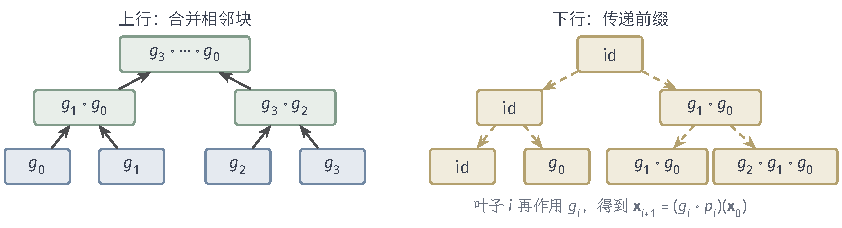
\includegraphics[width=150mm]{figures/03-optimization-evolution-and-signals/02-processes-and-trajectory-evolution/tikz/dds-parallel-scan/figure.pdf}
  \caption{四步仿射更新的关联扫描。左：上行阶段把相邻更新两两复合，每个节点保存所辖区间的总映射，较晚的更新始终写在左边。右：下行阶段从根传入恒等映射，左孩子继承父节点的前缀，右孩子接收“左兄弟的总映射$\circ$父节点前缀”。四个叶子得到的前缀依次是$\mathrm{id}$、$g_0$、$g_1\circ g_0$、$g_2\circ g_1\circ g_0$。同一层的合并互不依赖，可以同时进行。}
  \label{fig:dds-parallel-scan}
\end{figure*}

代价要分开计算。总工作量数所有节点上执行的合并次数，计算深度数最长依赖链上的合并次数。$T$步形成的平衡树有$O(T)$个节点、$O(\log T)$层，上行和下行在每个节点只做常数次合并，同层节点互不依赖。所以把一次合并算作一个操作时，总工作量为$O(T)$，\term{并行深度}（parallel depth）为$O(\log T)$，而顺序递推的深度是$T$。但一次合并的实际算术量取决于矩阵形式：一般稠密的$d\times d$矩阵相乘需要$O(d^3)$次运算，而顺序递推每步只需$O(d^2)$的矩阵乘向量，所以扫描用更多的总运算换取更短的深度。若$\bm A_n$都是对角矩阵，合并只需$O(d)$次运算，两种做法的总量同阶。线性状态空间序列模型常把转移矩阵取成对角形式并用这种扫描训练，原因即在于此\scite{gu2023mamba}。扫描还要保存树上的中间二元组，存储量为$O(T)$个二元组。

两点限制需要记住。第一，结合律保证的是精确算术下的结果相同，浮点运算改变括号会改变舍入：双精度下$(1+10^{17})-10^{17}=0$，而$1+(10^{17}-10^{17})=1$。长乘积或条件数较大的传播尤其敏感，所以并行实现应按误差容限验证，不能要求与顺序递推逐位相同。第二，扫描要求每一步的$(\bm A_n,\bm b_n)$事先已知。若系数依赖尚未算出的状态，例如$\bm A_n=\bm A(\bm x_n)$，就不能预先组成二元组；若复合后不再有固定大小的表示，压缩整段更新的前提也就不存在。
